\subsection{Simulation des Greifarms\hfill\textnormal{\emph{Berger}}}
Die Aufgabe dieser Implementierung war es
zu bestimmen in welcher Position die Gelenke eines Roboterarmes 
seien müssen um mit der Spitze eine bestimmte Zielposition zu erreichen.
Das Verfahren um dies zu berechnen nennt sich "Inverse Kinematik".

Für Python gibt es das ikpy-Package das genau dies umsetzt.
\footnote{https://github.com/Phylliade/ikpy}
Für die Berechnung werden jedoch zuerst Informationen über den Roboterarm benötigt.
Dies Beinhaltet die Ansatzpunkte der Arm-Elemente sowie die Art des Gelenke, 
zum Beispiel kippen oder drehen.
Diese Daten könnten manuell erstellt werden, 
was viel Zeit in Anspruch nehmen würde.
Deshalb wurde hierfür die Solidworks-Erweiterung URDF-Exporter benutzt.
\footnote{http://wiki.ros.org/sw\_urdf\_exporter}

Diese ermöglicht alle nötigen Informationen automatisch zu generieren.
Dazu werden alle relevanten Bauteile des Modells ausgewählt
und die Erweiterung erkennt nun die Rotationsachsen der Verbindungen 
und die Distanz und Position der Gelenke.
Diese Daten werden dann im URDF als exportiert,
was für "Unified Robot Description Format" steht 
eine weit verbreitete XML-Spezifikation ist.\cite{mathWorks}
\\

Unser Python-Skript generiert dann mit Hilfe des ikpy Package
aus den URDF-Daten eine sogenannte "Chain".
Eine zweite Funktion nimmt diese Chain und ein Array mit Koordinaten entgegen
und gibt die Ausrichtung der Kettenglieder aus.
Diese ausgerichtete Kette kann dann, 
wie in Abbildung \ref{fig:greifarm1} dargestellt,
mit dem Matplotlib-Package visualisiert werden.

\begin{figure}[H]
  \centering{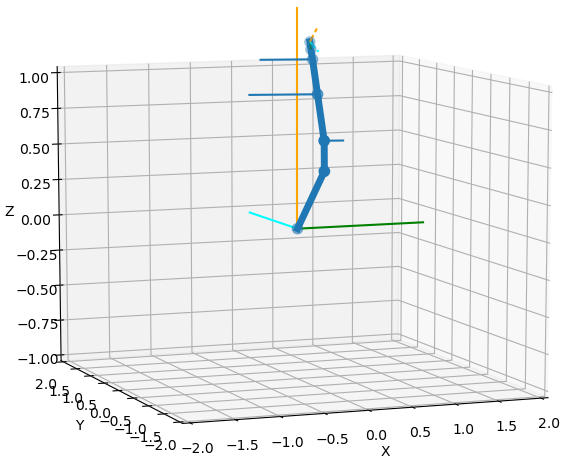
\includegraphics[width=1.0\linewidth]{Abbildungen/greifarm1.png}}
  \caption{Matplotlib ouput}
  \label{fig:greifarm1}
\end{figure}

Alternativ könnten diese Daten auch an einen tatsächlichen Roboter-Arm weitergegeben werden.
Der Rescue-Robot müsste nur die relative Position des zu greifenden Objekts berechnen
und könnte dann das Objekt greifen und dann eine Position über dem Container anfahren.

Zum jetzigen Zeitpunkt gibt es noch einige Probleme mit der Kette,
die wahrscheinlich an einer falschen Anwendung der Solidworks-Erweiterung liegen.
